\documentclass{beamer}
\usetheme{Warsaw}
\usecolortheme{beaver}
\usepackage{graphicx}

\title{Git user group \#1}
\subtitle{Introduction to git}
\author[Keruspe]{Marc-Antoine Perennou}
\institute[CC]{Clever Cloud}
\date{}

\begin{document}

\begin{frame}[plain]
    \titlepage
\end{frame}

\begin{frame}{Who I am}
    Marc-Antoine Perennou - 
\includegraphics[width=80px,height=30px]{logo-cc.png} \\
    \ \\
    \ \\
    \hrule
    \ \\
    \ \\
    Marc-Antoine@Perennou.com \\
    marc-antoine.perennou@clever-cloud.com \\
    \ \\
    \ \\
    \hrule
    \ \\
    \ \\
    http://clever-cloud.com/ \\
    @Keruspe on twitter and identi.ca \\
    http://github.com/Keruspe
\end{frame}

\begin{frame}{The (D)VCS concept}
    \begin{itemize}
        \item What is a Version Control System ?
        \pause
        \item Why must you use one if you do not do so already ?
        \pause
        \item Why should you consider using or switching to a Distributed VCS ?
    \end{itemize}
    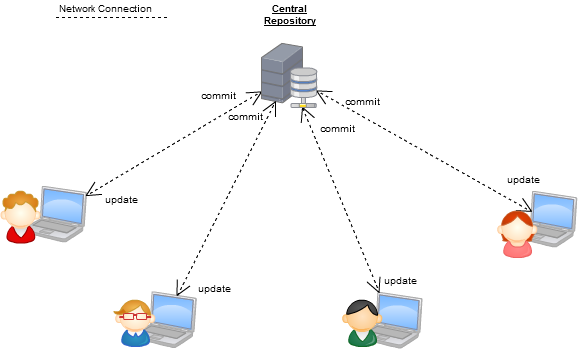
\includegraphics[width=130pt,height=100pt]{VCS.png} \ \vrule \ \
    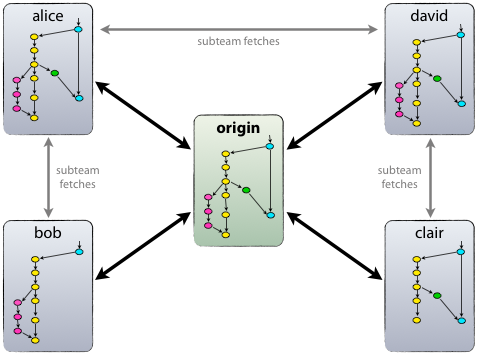
\includegraphics[width=130pt,height=100pt]{DVCS.png} \\
    \ \ \ \ \ \ \ \ \ \ \ \ \ \ \ \ VCS\ \ \ \ \ \ \ \ \ \ \ \ VS\ \ \ \ \ \ \ \ \ \ \ \ \ \ DVCS
\end{frame}

\begin{frame}{The origin of Git}
    
\includegraphics[width=60pt,height=30pt]{git-scm-logo.png}
    \begin{itemize}
        \item The creation of git
        \begin{itemize}
            \item Linux development constraints (Too many developers, thousands per year)
            \item First release: 1995
        \end{itemize}
        \pause
        \item The origin of its name
        \pause
        \item The evolution/complexification and usage simplification of git
    \end{itemize}
\end{frame}

\begin{frame}{Creating a repository}
    One command: git init\\
    This command creates the basic files needed by git into a subdirectory named ".git" \\
    \ \\
    \ \\
    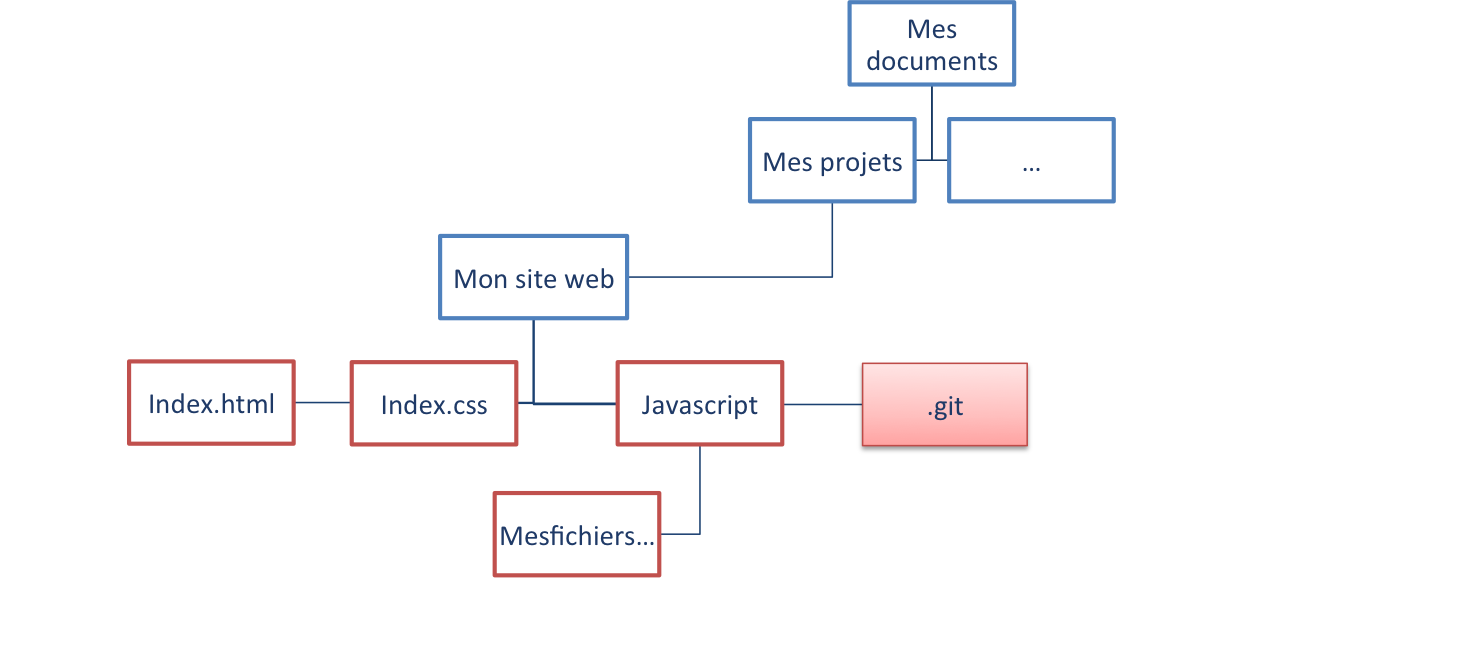
\includegraphics[width=250pt,height=110pt]{fileinit.png}
\end{frame}

\begin{frame}{Basic usage}
    5 mandatory commands : \\
    \begin{itemize}
        \item git init
        \item git clone
        \item git commit
        \item git push
        \item git pull
    \end{itemize}
    With those commands (and eventually git remote), you can act with git at least like you acted with SVN (for example)
\end{frame}

\begin{frame}{Git server side}
    \begin{itemize}
        \item Introduction to github
        \pause
        \item Demonstration: sharing this presentation on github
        \pause
        \item For your company: gitolite
        \pause
        \item Git with non-git backend
    \end{itemize}
\end{frame}

\begin{frame}{Some usefull basics}
    \begin{itemize}
        \item Explanations on the tracking system
        \pause
        \item Configuration
        \pause
        \item Editing the last commit
        \pause
        \item Cleaning a working tree
    \end{itemize}
\end{frame}

\begin{frame}{Branching}
    Three commands: \\
    \begin{itemize}
        \item git branch
        \item git checkout
        \item git merge
    \end{itemize}
    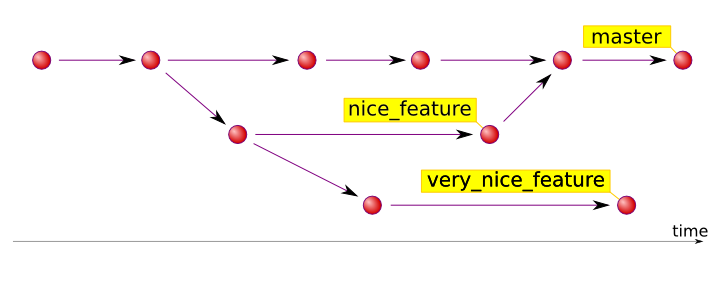
\includegraphics[width=300pt,height=130pt]{branches.png}
\end{frame}

\begin{frame}{Advanced usage}
    \begin{itemize}
        \item Rebasing with git rebase / git pull --rebase
        \pause
        \item Patching with git format-patch and git am
        \pause
        \item Backporting with git cherry-pick for maintainance
        \pause
        \item Debugging with git bisect
        \pause
        \item Tagging releases
        \pause
        \item Blaming colleagues
    \end{itemize}
\end{frame}

\begin{frame}{Demos}
    \begin{itemize}
        \item Failing merge
        \pause
        \item Successfull merge
        \pause
        \item paludis patches
        \pause
        \item play patches
        \pause
        \item Backporting changes
    \end{itemize}
\end{frame}

\end{document}

